%-------------------------------------------------------------
\subsection{Introducing graphs}
%-------------------------------------------------------------

%-------------------------------------------------------------
\begin{frame}[fragile]\frametitle{Plan}

\blue{What are graphs, how to represent them?}
\begin{itemize}
\item Concrete representation of graphs in maths
\item Representation of graphs in Haskell
\item Path search in concrete graphs
\end{itemize}

\blue{Different search strategies}
\begin{itemize}
\item depth-first
\item breadth-first
\end{itemize}

\blue{Abstract graphs}
\begin{itemize}
\item How to describe graphs without generating them explicitly
\item Searching for solutions in abstract graphs
\end{itemize}

\end{frame}

%-------------------------------------------------------------
\begin{frame}[fragile]\frametitle{A graph}

\begin{center}
\begin{tikzpicture}[scale=2,
on grid,
simple/.style ={shape=circle, fill=grey!50},
blue/.style ={shape=circle, fill=blue!50},
red/.style ={shape=circle, fill=red!50},
auto]

\node[simple] (a) at (0, 1) {A};
\node[simple] (b) at (1, 1) {B};
\node[simple] (c) at (2, 1) {C};
\node[simple] (d) at (0, -1) {D};
\node[simple] (e) at (1, 0) {E};
\node[simple] (f) at (3, 2) {F};
\node[simple] (g) at (1, 2) {G};
\node[simple] (h) at (2, -1) {H};
\node[simple] (i) at (3, 0) {I};
\node[simple] (j) at (3, 1) {J};

\begin{scope}[every path/.style=solid,thick]
\draw[->] (a) -- (b);
\draw[->] (a) -- (d);
\draw[->] (b) -- (c);
\draw[->] (b) -- (g);
\draw[->] (a) -- (e);
\draw[->] (c) -- (i);
\draw[->] (c) -- (f);
\draw[->] (c) -- (g);
\draw[->] (d) -- (h);
\draw[->] (e) -- (i);
\draw[->] (e) -- (h);
\draw[->] (i) -- (j);
\draw[->] (f) -- (j);
\end{scope}
\end{tikzpicture}
\end{center}


%%% Local Variables: 
%%% mode: latex
%%% TeX-master: "../main_recherche"
%%% End: 


\end{frame}


%-------------------------------------------------------------
\begin{frame}[fragile]\frametitle{Some other graphs}

\begin{columns}[t]
\column{.5\textwidth}

\blue{Metro / bus network (in Toulouse)}
\begin{center}
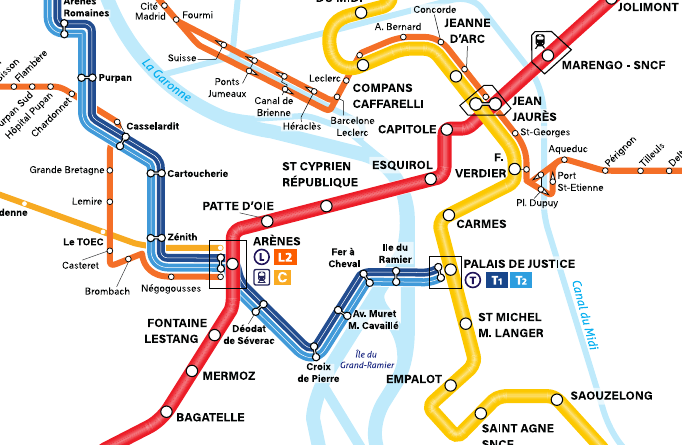
\includegraphics[scale=0.3]{Figures/reseau_tisseo.png}
\end{center}

\column{.5\textwidth}
\blue{Internet} (Arpanet, 1977)
\begin{center}
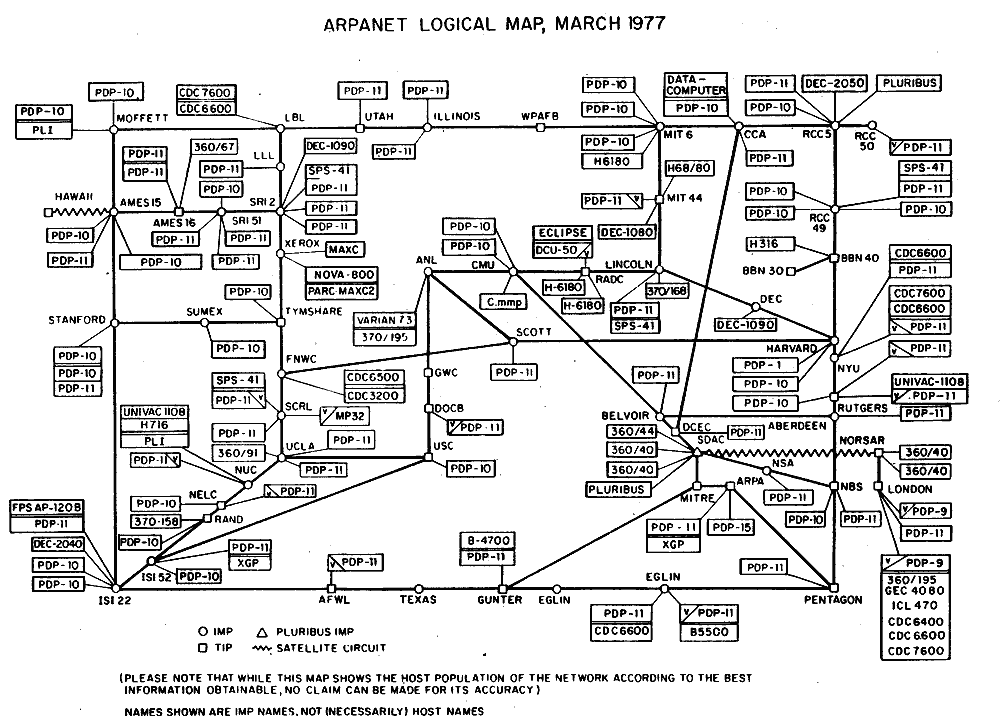
\includegraphics[scale=0.18]{Figures/arpanet_logical_map_1977.png}

\tiny{source: \url{https://en.wikipedia.org/wiki/ARPANET}}
\end{center}

\end{columns}

\end{frame}



%-------------------------------------------------------------
\begin{frame}[fragile]\frametitle{Graphs - mathematically}

  A \blue{directed graph} is defined as a couple $G = (V, E)$ where:
  \begin{itemize}
  \item $V$ is a set of vertices
  \item $E \subseteq V \times V$ is a set of edges
  \end{itemize}

  \vspace{5mm}
\begin{columns}[t]
  \column{.4\textwidth}
  \begin{center}
\begin{tikzpicture}[scale=1.5,
on grid,
simple/.style ={shape=circle, fill=grey!50},
blue/.style ={shape=circle, fill=blue!50},
red/.style ={shape=circle, fill=red!50},
auto]

\node[simple] (a) at (0, 1) {A};
\node[simple] (b) at (1, 1) {B};
\node[simple] (c) at (2, 1) {C};
\node[simple] (g) at (1, 2) {G};

\begin{scope}[every path/.style=solid,thick]
\draw[->] (a) -- (b);
\draw[->] (b) -- (c);
\draw[->] (b) -- (g);
\draw[<->] (c) -- (g);
\end{scope}
\end{tikzpicture}
\end{center}
  \column{.6\textwidth}
  \emph{Here:}
  \begin{itemize}
  \item $V = \{A, B, C, G\}$
  \item $E = \{(A, B), (B, C), (B, G), (C, G), (G, C) \}$
  \item \emph{Possible} to walk from $A$ to $G$
  \item \emph{Impossible} to walk from $G$ to $A$
  \end{itemize}
\end{columns}

\end{frame}


%-------------------------------------------------------------
\begin{frame}[fragile]\frametitle{Graphs - mathematically}

\emph{Variant:} An \blue{undirected graph} is a graph where the edge relation
is bidirectional (symetric).\\
$\leadsto$ useless to draw arrow heads

  \vspace{5mm}
\begin{columns}[t]
  \column{.45\textwidth}
  \begin{center}
\begin{tikzpicture}[scale=1.5,
on grid,
simple/.style ={shape=circle, fill=grey!50},
blue/.style ={shape=circle, fill=blue!50},
red/.style ={shape=circle, fill=red!50},
auto]

\node[simple] (a) at (0, 1) {A};
\node[simple] (b) at (1, 1) {B};
\node[simple] (c) at (2, 1) {C};
\node[simple] (g) at (1, 2) {G};

\begin{scope}[every path/.style=solid,thick]
\draw[-] (a) -- (b);
\draw[-] (b) -- (c);
\draw[-] (b) -- (g);
\draw[-] (c) -- (g);
\end{scope}
\end{tikzpicture}
\end{center}
  \column{.55\textwidth}
  \emph{Here:}
  \begin{itemize}
  \item $V = \{A, B, C, G\}$
  \item $E = \{(A, B), (B, A), (B, C), (C, B),$
    $(B, G), (G, B), (C, G), (G, C) \}$
  \item \emph{Possible} to walk from $A$ to $G$
  \item \dots{} and back
  \end{itemize}
\end{columns}

\emph{Note:}
\begin{itemize}
\item Undirected graphs can always be reduced to directed graphs\\
  (by making the edge relation symetric)
\item \dots{} and thus will not be considered explicitly
\end{itemize}

\end{frame}




%-------------------------------------------------------------
\begin{frame}[fragile]\frametitle{Edge-Labelled Graphs}

  It might be useful to label edges to indicate:
  \begin{itemize}
  \item costs (of traversing an edge)
  \item capacity (transport, pipeline)
  \item action (triggered by traversal)
  \end{itemize}


  \vspace{5mm}
\begin{columns}[t]
  \column{.45\textwidth}
  \begin{center}
    \begin{tikzpicture}[scale=1.5,
on grid,
simple/.style ={shape=circle, fill=grey!50},
blue/.style ={shape=circle, fill=blue!50},
red/.style ={shape=circle, fill=red!50},
auto]

\node[simple] (a) at (0, 1) {A};
\node[simple] (b) at (1, 1) {B};
\node[simple] (c) at (2, 1) {C};
\node[simple] (g) at (1, 2) {G};

\begin{scope}[every path/.style=solid,thick]
\draw[->] (a) to node {3} (b);
\draw[->] (b) to node {4} (c);
\draw[->] (b) to node {2} (g);
\draw[<->] (g) to node {5} (c);
\end{scope}
\end{tikzpicture}

%%% Local Variables:
%%% mode: latex
%%% TeX-master: "../main"
%%% End:

  \end{center}
  \column{.55\textwidth}
  \emph{Possible representation:} as triple:
  \begin{itemize}
  \item $V = \{A, B, C, G\}$
  \item $E = \{(A, B, 3), (B, C, 4),$
    $(B, G, 2), (C, G, 5), (G, C, 5) \}$
  \end{itemize}
\end{columns}

\end{frame}


%-------------------------------------------------------------
\begin{frame}[fragile]\frametitle{Automata}

  Automata are particular kinds of edge-labelled graphs, typically with:
  \begin{itemize}
  \item one start node
  \item one or several goal nodes
  \end{itemize}

  
\begin{columns}[t]
  \column{.5\textwidth}

  \usetikzlibrary {automata,positioning}
\begin{tikzpicture}[scale=0.8,shorten >=1pt,node distance=2cm,on grid,auto]
\node[state,initial] (q_0)
 {$q_0$};
\node[state]
 (q_1) [above right=of q_0]
 {$q_1$};
\node[state]
 (q_2) [below right=of q_0]
 {$q_2$};
\node[state,accepting](q_3) [below right=of q_1]
 {$q_3$};
\path[->] (q_0) edge
 node
 {0} (q_1)
edge
 node [swap] {1} (q_2)
(q_1) edge
 node
 {1} (q_3)
edge [loop above]
 node
 {0} ()
(q_2) edge
 node [swap] {0} (q_3)
edge [loop below]
 node
 {1} ();
\end{tikzpicture}

\column{.5\textwidth}

Admissible runs of the automaton:
\begin{itemize}
\item 01, 001, \dots, 0(0*)1
\item 10, 110, \dots, 1(1*)0
\end{itemize}

\end{columns}

\end{frame}



%-------------------------------------------------------------
\subsection{Graphs in Haskell}
%-------------------------------------------------------------


%-------------------------------------------------------------
\begin{frame}[fragile]\frametitle{Graphs Library in Haskell}

  \begin{itemize}
  \item Package \texttt{fgl} (Martin Erwig's Functional Graph Library):
    \url{https://hackage.haskell.org/package/fgl}

  \item in \texttt{Data.Graph.Inductive.Graph}:
    \begin{lstlisting}
      class Graph gr
    \end{lstlisting}    

  \item Two instances \texttt{Graph Gr}:
    \begin{itemize}
    \item \texttt{Data.Graph.Inductive.PatriciaTree} (used here)
    \item \texttt{Data.Graph.Inductive.Tree}
    \end{itemize}
    
  \end{itemize}

\end{frame}


%-------------------------------------------------------------
\begin{frame}[fragile]\frametitle{Haskell: ``simple'' graphs}

  Node type: synonym of Integer; Edges: couples of nodes

\begin{lstlisting}
  type Node = Int
  type Edge = (Node, Node)
\end{lstlisting}
  
Required for constructing a graph: Labelled nodes and edges

\begin{lstlisting}
  type LNode a = (Node, a)
  type LEdge b = (Node, Node, b) 
\end{lstlisting}

\end{frame}

%-------------------------------------------------------------
\begin{frame}[fragile]\frametitle{Haskell: ``simple'' graphs}

Constructing the graph:
\small
\begin{lstlisting}
import Data.Graph.Inductive.Graph
import Data.Graph.Inductive.PatriciaTree
  
smallGrNodes :: [LNode String]
smallGrNodes = [(0, "A"), (1, "B"), (2, "C"), (3, "G")]

smallGrEdges :: [LEdge Int]
smallGrEdges = [(0, 1, 3), (1, 2, 4), (1, 3, 2),
                (2, 3, 5), (3, 2, 5)]

smallGraph :: Gr String Int
smallGraph = mkGraph smallGrNodes smallGrEdges
\end{lstlisting}
\normalsize
\end{frame}


%-------------------------------------------------------------
\begin{frame}[fragile]\frametitle{Introducing Graphviz}

\begin{columns}[t]
  \column{.5\textwidth}
  \blue{Graphviz}  (\url{http://graphviz.org/})
  \begin{itemize}
  \item An expressive graph description language
  \item rather unreadable ``as such'' 
  \item display in browser: \url{https://dreampuf.github.io/GraphvizOnline/}
  \item convertible to many display formats (png, pdf, \dots)
  \end{itemize}
  \column{.5\textwidth}
\tiny
\begin{verbatim}
digraph {
    subgraph cluster_0 {
        graph [label=IN
              ,labeljust=l
              ,style=invis];
        1 [label=OrderBike];
        4 [label=ReceivesPay];
        6 [label=AwaitDeliverBike];
        12 [label=AwaitBuyerPays];   }
    subgraph cluster_1 {
        graph [label=OUT
              ,labeljust=r
              ,style=invis];
        17 [label=BREACH];
        18 [label=FULFILLED];    }
    1 -> 6 [headport=n
           ,tailport=se
           ,color=blue];
    1 -> 18 [headport=n
            ,tailport=sw
            ,color=brown];
    12 -> 17 [headport=n
             ,tailport=sw
             ,color=brown];
    12 -> 18 [headport=n
             ,tailport=se
             ,color=blue];
}
\end{verbatim}
\normalsize
\end{columns}

\end{frame}


%-------------------------------------------------------------
\begin{frame}[fragile]\frametitle{Displaying graphs with Graphviz}

Use Haskell Graphviz package (\url{https://hackage.haskell.org/package/graphviz})

\begin{itemize}
\item to convert graphs to Graphviz, or
\item to bypass Graphviz and directly produce a PDF
\end{itemize}


\small
\begin{lstlisting}
import Data.GraphViz
import Data.GraphViz.Printing
import Data.GraphViz.Commands
import Data.GraphViz.Attributes.Complete

smallGrDot :: IO FilePath
smallGrDot = runGraphviz
       (graphToDot quickParams smallGraph) Pdf "graph.pdf"
\end{lstlisting}
\normalsize

Run \texttt{smallGrDot}
\end{frame}


%-------------------------------------------------------------
\begin{frame}[fragile]\frametitle{Displaying graphs with Graphviz}

  Compare:

  \begin{columns}[t]
    \column{.5\textwidth}
    \vspace{2cm}
  \begin{center}
    \begin{tikzpicture}[scale=1.5,
on grid,
simple/.style ={shape=circle, fill=grey!50},
blue/.style ={shape=circle, fill=blue!50},
red/.style ={shape=circle, fill=red!50},
auto]

\node[simple] (a) at (0, 1) {A};
\node[simple] (b) at (1, 1) {B};
\node[simple] (c) at (2, 1) {C};
\node[simple] (g) at (1, 2) {G};

\begin{scope}[every path/.style=solid,thick]
\draw[->] (a) to node {3} (b);
\draw[->] (b) to node {4} (c);
\draw[->] (b) to node {2} (g);
\draw[<->] (g) to node {5} (c);
\end{scope}
\end{tikzpicture}

%%% Local Variables:
%%% mode: latex
%%% TeX-master: "../main"
%%% End:

  \end{center}
  \column{.5\textwidth}
  \begin{center}
    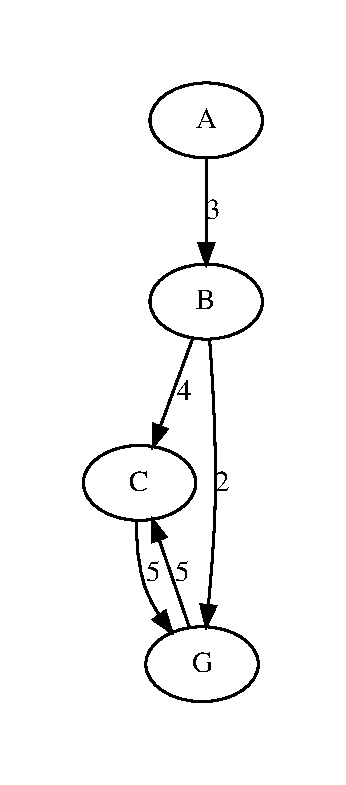
\includegraphics[scale=0.5]{Figures/small_graph_gen_graphviz.pdf}
  \end{center}
\end{columns}

\end{frame}



%-------------------------------------------------------------
\begin{frame}[fragile]\frametitle{Using the Haskell Graphs Library}

  Functions for:

  \begin{itemize}
  \item constructing a graph progressively 
  \item decomposing a graph into node, adjacent edges ``and the rest''
  \item \dots
  \end{itemize}

  What is nice about the graph library:
  \begin{itemize}
  \item efficient implementation
  \end{itemize}

  What is not nice:
  \begin{itemize}
  \item you have to address nodes by their IDs
  \item impossible to address nodes by their labels \\
    (OK, these might be ambiguous)
  \item $\leadsto$ dictionary translating between IDs and labels
  \end{itemize}
\end{frame}




%-------------------------------------------------------------
\subsection{Path search in a concrete graph}
%-------------------------------------------------------------



%-------------------------------------------------------------
\begin{frame}[fragile]\frametitle{Path search}

\blue{Intention:} Search for a path from the \emph{start} node to a
\emph{goal} node.

\blue{Here:}

\begin{itemize}
\item \emph{Path}: sequence of nodes: start -  intermediate - goal
\item Particularities of the graph:
  \begin{itemize}
  \item Directed graph
  \item No edge labelling
  \end{itemize}
\item Possibly look for several solutions.
\item Can we aim at \emph{all} solutions?
\end{itemize}

\end{frame}

%-------------------------------------------------------------
\begin{frame}[fragile]\frametitle{Depth-First Search, DFS (1)}

\begin{columns}[t]
\column{.6\textwidth}

\begin{onlyenv}<1>
\begin{center}
\begin{tikzpicture}[scale=1.5,
on grid,
simple/.style ={shape=circle, fill=grey!50},
blue/.style ={shape=circle, fill=blue!50},
red/.style ={shape=circle, fill=red!50},
auto]

\node[red] (a) at (0, 1) {A};
\node[simple] (b) at (1, 1) {B};
\node[simple] (c) at (2, 1) {C};
\node[simple] (d) at (0, -1) {D};
\node[simple] (e) at (1, 0) {E};
\node[simple] (f) at (3, 2) {F};
\node[simple] (g) at (1, 2) {G};
\node[simple] (h) at (2, -1) {H};
\node[simple] (i) at (3, 0) {I};
\node[simple] (j) at (3, 1) {J};

\begin{scope}[every path/.style=solid,thick]
\draw[->] (a) -- (b);
\draw[->] (a) -- (d);
\draw[->] (b) -- (c);
\draw[->] (b) -- (g);
\draw[->] (a) -- (e);
\draw[->] (c) -- (i);
\draw[->] (c) -- (f);
\draw[->] (c) -- (g);
\draw[->] (d) -- (h);
\draw[->] (e) -- (i);
\draw[->] (e) -- (h);
\draw[->] (i) -- (j);
\draw[->] (f) -- (j);
\end{scope}
\end{tikzpicture}
\end{center}


%%% Local Variables: 
%%% mode: latex
%%% TeX-master: "../main_recherche"
%%% End: 

\end{onlyenv}
\begin{onlyenv}<2>
\begin{center}
\begin{tikzpicture}[scale=1.5,
on grid,
simple/.style ={shape=circle, fill=grey!50},
blue/.style ={shape=circle, fill=blue!50},
red/.style ={shape=circle, fill=red!50},
auto]

\node[simple] (a) at (0, 1) {A};
\node[red] (b) at (1, 1) {B};
\node[simple] (c) at (2, 1) {C};
\node[blue] (d) at (0, -1) {D};
\node[blue] (e) at (1, 0) {E};
\node[simple] (f) at (3, 2) {F};
\node[simple] (g) at (1, 2) {G};
\node[simple] (h) at (2, -1) {H};
\node[simple] (i) at (3, 0) {I};
\node[simple] (j) at (3, 1) {J};

\begin{scope}[every path/.style=solid,thick]
\draw[->] (a) -- (b);
\draw[->] (a) -- (d);
\draw[->] (b) -- (c);
\draw[->] (b) -- (g);
\draw[->] (a) -- (e);
\draw[->] (c) -- (i);
\draw[->] (c) -- (f);
\draw[->] (c) -- (g);
\draw[->] (d) -- (h);
\draw[->] (e) -- (i);
\draw[->] (e) -- (h);
\draw[->] (i) -- (j);
\draw[->] (f) -- (j);
\end{scope}
\end{tikzpicture}
\end{center}


%%% Local Variables: 
%%% mode: latex
%%% TeX-master: "../main_recherche"
%%% End: 

\end{onlyenv}
\begin{onlyenv}<3>
\begin{center}
\begin{tikzpicture}[scale=1.5,
on grid,
simple/.style ={shape=circle, fill=grey!50},
blue/.style ={shape=circle, fill=blue!50},
red/.style ={shape=circle, fill=red!50},
auto]

\node[simple] (a) at (0, 1) {A};
\node[simple] (b) at (1, 1) {B};
\node[red] (c) at (2, 1) {C};
\node[blue] (d) at (0, -1) {D};
\node[blue] (e) at (1, 0) {E};
\node[simple] (f) at (3, 2) {F};
\node[blue] (g) at (1, 2) {G};
\node[simple] (h) at (2, -1) {H};
\node[simple] (i) at (3, 0) {I};
\node[simple] (j) at (3, 1) {J};

\begin{scope}[every path/.style=solid,thick]
\draw[->] (a) -- (b);
\draw[->] (a) -- (d);
\draw[->] (b) -- (c);
\draw[->] (b) -- (g);
\draw[->] (a) -- (e);
\draw[->] (c) -- (i);
\draw[->] (c) -- (f);
\draw[->] (c) -- (g);
\draw[->] (d) -- (h);
\draw[->] (e) -- (i);
\draw[->] (e) -- (h);
\draw[->] (i) -- (j);
\draw[->] (f) -- (j);
\end{scope}
\end{tikzpicture}
\end{center}


%%% Local Variables: 
%%% mode: latex
%%% TeX-master: "../main_recherche"
%%% End: 

\end{onlyenv}
\begin{onlyenv}<4>
\begin{center}
\begin{tikzpicture}[scale=1.5,
on grid,
simple/.style ={shape=circle, fill=grey!50},
blue/.style ={shape=circle, fill=blue!50},
red/.style ={shape=circle, fill=red!50},
auto]

\node[simple] (a) at (0, 1) {A};
\node[simple] (b) at (1, 1) {B};
\node[simple] (c) at (2, 1) {C};
\node[blue] (d) at (0, -1) {D};
\node[blue] (e) at (1, 0) {E};
\node[blue] (f) at (3, 2) {F};
\node[red] (g) at (1, 2) {G};
\node[simple] (h) at (2, -1) {H};
\node[blue] (i) at (3, 0) {I};
\node[simple] (j) at (3, 1) {J};

\begin{scope}[every path/.style=solid,thick]
\draw[->] (a) -- (b);
\draw[->] (a) -- (d);
\draw[->] (b) -- (c);
\draw[->] (b) -- (g);
\draw[->] (a) -- (e);
\draw[->] (c) -- (i);
\draw[->] (c) -- (f);
\draw[->] (c) -- (g);
\draw[->] (d) -- (h);
\draw[->] (e) -- (i);
\draw[->] (e) -- (h);
\draw[->] (i) -- (j);
\draw[->] (f) -- (j);
\end{scope}
\end{tikzpicture}
\end{center}


%%% Local Variables: 
%%% mode: latex
%%% TeX-master: "../main_recherche"
%%% End: 

\end{onlyenv}
\begin{onlyenv}<5>
\begin{center}
\begin{tikzpicture}[scale=1.5,
on grid,
simple/.style ={shape=circle, fill=grey!50},
blue/.style ={shape=circle, fill=blue!50},
red/.style ={shape=circle, fill=red!50},
auto]

\node[simple] (a) at (0, 1) {A};
\node[simple] (b) at (1, 1) {B};
\node[simple] (c) at (2, 1) {C};
\node[blue] (d) at (0, -1) {D};
\node[blue] (e) at (1, 0) {E};
\node[red] (f) at (3, 2) {F};
\node[blue] (g) at (1, 2) {G};
\node[simple] (h) at (2, -1) {H};
\node[blue] (i) at (3, 0) {I};
\node[simple] (j) at (3, 1) {J};

\begin{scope}[every path/.style=solid,thick]
\draw[->] (a) -- (b);
\draw[->] (a) -- (d);
\draw[->] (b) -- (c);
\draw[->] (b) -- (g);
\draw[->] (a) -- (e);
\draw[->] (c) -- (i);
\draw[->] (c) -- (f);
\draw[->] (c) -- (g);
\draw[->] (d) -- (h);
\draw[->] (e) -- (i);
\draw[->] (e) -- (h);
\draw[->] (i) -- (j);
\draw[->] (f) -- (j);
\end{scope}
\end{tikzpicture}
\end{center}


%%% Local Variables: 
%%% mode: latex
%%% TeX-master: "../main_recherche"
%%% End: 

\end{onlyenv}
\begin{onlyenv}<6>
\begin{center}
\begin{tikzpicture}[scale=1.5,
on grid,
simple/.style ={shape=circle, fill=grey!50},
blue/.style ={shape=circle, fill=blue!50},
red/.style ={shape=circle, fill=red!50},
auto]

\node[simple] (a) at (0, 1) {A};
\node[simple] (b) at (1, 1) {B};
\node[simple] (c) at (2, 1) {C};
\node[blue] (d) at (0, -1) {D};
\node[blue] (e) at (1, 0) {E};
\node[simple] (f) at (3, 2) {F};
\node[blue] (g) at (1, 2) {G};
\node[simple] (h) at (2, -1) {H};
\node[blue] (i) at (3, 0) {I};
\node[red] (j) at (3, 1) {J};

\begin{scope}[every path/.style=solid,thick]
\draw[->] (a) -- (b);
\draw[->] (a) -- (d);
\draw[->] (b) -- (c);
\draw[->] (b) -- (g);
\draw[->] (a) -- (e);
\draw[->] (c) -- (i);
\draw[->] (c) -- (f);
\draw[->] (c) -- (g);
\draw[->] (d) -- (h);
\draw[->] (e) -- (i);
\draw[->] (e) -- (h);
\draw[->] (i) -- (j);
\draw[->] (f) -- (j);
\end{scope}
\end{tikzpicture}
\end{center}


%%% Local Variables: 
%%% mode: latex
%%% TeX-master: "../main_recherche"
%%% End: 

\end{onlyenv}
\begin{onlyenv}<7>
\begin{center}
\begin{tikzpicture}[scale=1.5,
on grid,
simple/.style ={shape=circle, fill=grey!50},
blue/.style ={shape=circle, fill=blue!50},
red/.style ={shape=circle, fill=red!50},
auto]

\node[simple] (a) at (0, 1) {A};
\node[simple] (b) at (1, 1) {B};
\node[simple] (c) at (2, 1) {C};
\node[blue] (d) at (0, -1) {D};
\node[blue] (e) at (1, 0) {E};
\node[simple] (f) at (3, 2) {F};
\node[blue] (g) at (1, 2) {G};
\node[simple] (h) at (2, -1) {H};
\node[red] (i) at (3, 0) {I};
\node[simple] (j) at (3, 1) {J};

\begin{scope}[every path/.style=solid,thick]
\draw[->] (a) -- (b);
\draw[->] (a) -- (d);
\draw[->] (b) -- (c);
\draw[->] (b) -- (g);
\draw[->] (a) -- (e);
\draw[->] (c) -- (i);
\draw[->] (c) -- (f);
\draw[->] (c) -- (g);
\draw[->] (d) -- (h);
\draw[->] (e) -- (i);
\draw[->] (e) -- (h);
\draw[->] (i) -- (j);
\draw[->] (f) -- (j);
\end{scope}
\end{tikzpicture}
\end{center}


%%% Local Variables: 
%%% mode: latex
%%% TeX-master: "../main_recherche"
%%% End: 

\end{onlyenv}
\begin{onlyenv}<8>
\begin{center}
\begin{tikzpicture}[scale=1.5,
on grid,
simple/.style ={shape=circle, fill=grey!50},
blue/.style ={shape=circle, fill=blue!50},
red/.style ={shape=circle, fill=red!50},
auto]

\node[simple] (a) at (0, 1) {A};
\node[simple] (b) at (1, 1) {B};
\node[simple] (c) at (2, 1) {C};
\node[blue] (d) at (0, -1) {D};
\node[blue] (e) at (1, 0) {E};
\node[simple] (f) at (3, 2) {F};
\node[blue] (g) at (1, 2) {G};
\node[simple] (h) at (2, -1) {H};
\node[simple] (i) at (3, 0) {I};
\node[red] (j) at (3, 1) {J};

\begin{scope}[every path/.style=solid,thick]
\draw[->] (a) -- (b);
\draw[->] (a) -- (d);
\draw[->] (b) -- (c);
\draw[->] (b) -- (g);
\draw[->] (a) -- (e);
\draw[->] (c) -- (i);
\draw[->] (c) -- (f);
\draw[->] (c) -- (g);
\draw[->] (d) -- (h);
\draw[->] (e) -- (i);
\draw[->] (e) -- (h);
\draw[->] (i) -- (j);
\draw[->] (f) -- (j);
\end{scope}
\end{tikzpicture}
\end{center}


%%% Local Variables: 
%%% mode: latex
%%% TeX-master: "../main_recherche"
%%% End: 

\end{onlyenv}

\column{.4\textwidth}
\blue{Look for} path A \dots J

\begin{onlyenv}<1>
\blue{Active state:} \red{A}
\end{onlyenv}

\begin{onlyenv}<2>
\blue{Active state:} A - \red{B}

\blue{On the stack:}
\begin{itemize}
\item  A - \blue{D}
\item  A - \blue{E}
\end{itemize}
\end{onlyenv}

\begin{onlyenv}<3>
\blue{Active state:} A - B - \red{C}

\blue{On the stack:}
\begin{itemize}
\item  A - B - \blue{G}
\item  A - \blue{D}
\item  A - \blue{E}
\end{itemize}
\end{onlyenv}

\begin{onlyenv}<4>
\blue{Active state:} A - B - C - \red{G}

\blue{On the stack:}
\begin{itemize}
\item  A - B  - C - \blue{F}
\item  A - B  - C - \blue{I}
\item  A - B - \blue{G}
\item  A - \blue{D}
\item  A - \blue{E}
\end{itemize}

$\leadsto$ backtrack
\end{onlyenv}

\begin{onlyenv}<5>
\blue{Active state:} A - B  - C - \red{F}

\blue{On the stack:}
\begin{itemize}
\item  A - B  - C - \blue{I}
\item  A - B - \blue{G}
\item  A - \blue{D}
\item  A - \blue{E}
\end{itemize}
\end{onlyenv}

\begin{onlyenv}<6>
\blue{Active state:} A - B - C - F - \red{J}

\blue{On the stack:}
\begin{itemize}
\item  A - B  - C - \blue{I}
\item  A - B - \blue{G}
\item  A - \blue{D}
\item  A - \blue{E}
\end{itemize}

\blue{Solutions:}
\begin{itemize}
\item  A - B - C - F - J
\end{itemize}
\end{onlyenv}

% \begin{onlyenv}<7>
% \blue{Active state:} A - B  - C - \red{I}

% \blue{On the stack:}
% \begin{itemize}
% \item  A - B - \blue{G}
% \item  A - \blue{D}
% \item  A - \blue{E}
% \end{itemize}

% \blue{Solutions:}
% \begin{itemize}
% \item  A - B - C - F - J
% \end{itemize}
% \end{onlyenv}

\begin{onlyenv}<7>
\blue{Active state:} A - B  - C - \red{I}

\blue{On the stack:}
\begin{itemize}
\item  A - B - \blue{G}
\item  A - \blue{D}
\item  A - \blue{E}
\end{itemize}

\blue{Solutions:}
\begin{itemize}
\item  A - B - C - F - J
\end{itemize}
\end{onlyenv}

\begin{onlyenv}<8>
\blue{Active state:} A - B  - C - I - \red{J}

\blue{On the stack:}
\begin{itemize}
\item  A - B - \blue{G}
\item  A - \blue{D}
\item  A - \blue{E}
\end{itemize}

\blue{Solutions:}
\begin{itemize}
\item  A - B - C - F - J
\item  A - B - C - I - J
\end{itemize}

\red{etc.}
\end{onlyenv}

\end{columns}


\end{frame}

%-------------------------------------------------------------
\begin{frame}[fragile]\frametitle{Depth-First-Search, DFS (2)}

\blue{Data structure:}

\begin{itemize}
\item notion of \emph{state}: partial path from the start to the goal
\item one state is \emph{active}
\item stack of partial solutions
\item a list of solutions
\end{itemize}

\blue{Principles:}
\begin{itemize}
\item if the stack is empty, stop the search
\item otherwise:
  \begin{itemize}
  \item if the active state is the goal, add state to solution set;\\
    then restart with next element on stack
  \item if the active state is not a goal, explore one successor state\\
    put remaining successors on stack
  \end{itemize}
\end{itemize}

\end{frame}



%-------------------------------------------------------------
\begin{frame}[fragile]\frametitle{Depth-First-Search, DFS (3)}

\emph{Exercise:} look for paths from A \dots H:


\begin{columns}[t]
\column{.5\textwidth}
\begin{center}
\begin{tikzpicture}[scale=1.5,
on grid,
simple/.style ={shape=circle, fill=grey!50},
colored/.style ={shape=circle, fill=red!50},
auto]

\node[simple] (a) at (0, 1) {A};
\node[simple] (b) at (1, 1) {B};
\node[simple] (c) at (2, 1) {C};
\node[simple] (d) at (0, -1) {D};
\node[simple] (e) at (1, 0) {E};
\node[simple] (f) at (2, 0) {F};
\node[simple] (g) at (1, 2) {G};
\node[simple] (h) at (2, -1) {H};

\begin{scope}[every path/.style=solid,thick]
\draw[->] (a) -- (b);
\draw[->] (a) -- (d);
\draw[->] (b) -- (c);
\draw[->] (b) -- (g);
\draw[->] (a) -- (e);
\draw[->] (c) -- (f);
\draw[->] (c) -- (g);
\draw[->] (d) -- (h);
\draw[->] (e) -- (d);
\draw[->] (e) -- (h);
\end{scope}
\end{tikzpicture}
\end{center}


%%% Local Variables: 
%%% mode: latex
%%% TeX-master: "../main_recherche"
%%% End: 


\column{.5\textwidth}
\begin{center}
\begin{tikzpicture}[scale=1.5,
on grid,
simple/.style ={shape=circle, fill=grey!50},
colored/.style ={shape=circle, fill=red!50},
auto]

\node[simple] (a) at (0, 1) {A};
\node[simple] (b) at (1, 1) {B};
\node[simple] (c) at (2, 1) {C};
\node[simple] (d) at (0, -1) {D};
\node[simple] (e) at (1, 0) {E};
\node[simple] (f) at (2, 0) {F};
\node[simple] (g) at (1, 2) {G};
\node[simple] (h) at (2, -1) {H};

\begin{scope}[every path/.style=solid,thick]
\draw[->] (a) -- (b);
\draw[->] (d) -- (a);
\draw[->] (b) -- (c);
\draw[->] (b) -- (g);
\draw[->] (a) -- (e);
\draw[->] (c) -- (f);
\draw[->] (c) -- (g);
\draw[->] (d) -- (h);
\draw[->] (e) -- (d);
\draw[->] (e) -- (h);
\end{scope}
\end{tikzpicture}
\end{center}


%%% Local Variables: 
%%% mode: latex
%%% TeX-master: "../main_recherche"
%%% End: 


\end{columns}

\end{frame}


%-------------------------------------------------------------
\begin{frame}[fragile]\frametitle{Breadth-First Search, BFS (1)}


  \blue{Data structure:}
  
\begin{itemize}
\item notion of \emph{state}: as for DFS
\item a list of active states
\item a list of solutions
\end{itemize}

\blue{Principles:}
\begin{itemize}
\item if the stack is empty, stop the search
\item otherwise:
  \begin{itemize}

  \item add the active states that correspond to goals to solution set
  \item replace active states by all possible successor states
  \end{itemize}
\end{itemize}

\end{frame}


%-------------------------------------------------------------
\begin{frame}[fragile]\frametitle{Breadth-First Search, BFS (2)}


\begin{columns}[t]
\column{.6\textwidth}

\begin{onlyenv}<1>
\begin{center}
\begin{tikzpicture}[scale=1.5,
on grid,
simple/.style ={shape=circle, fill=grey!50},
blue/.style ={shape=circle, fill=blue!50},
red/.style ={shape=circle, fill=red!50},
auto]

\node[red] (a) at (0, 1) {A};
\node[simple] (b) at (1, 1) {B};
\node[simple] (c) at (2, 1) {C};
\node[simple] (d) at (0, -1) {D};
\node[simple] (e) at (1, 0) {E};
\node[simple] (f) at (3, 2) {F};
\node[simple] (g) at (1, 2) {G};
\node[simple] (h) at (2, -1) {H};
\node[simple] (i) at (3, 0) {I};
\node[simple] (j) at (3, 1) {J};

\begin{scope}[every path/.style=solid,thick]
\draw[->] (a) -- (b);
\draw[->] (a) -- (d);
\draw[->] (b) -- (c);
\draw[->] (b) -- (g);
\draw[->] (a) -- (e);
\draw[->] (c) -- (i);
\draw[->] (c) -- (f);
\draw[->] (c) -- (g);
\draw[->] (d) -- (h);
\draw[->] (e) -- (i);
\draw[->] (e) -- (h);
\draw[->] (i) -- (j);
\draw[->] (f) -- (j);
\end{scope}
\end{tikzpicture}
\end{center}


%%% Local Variables: 
%%% mode: latex
%%% TeX-master: "../main_recherche"
%%% End: 

\end{onlyenv}
\begin{onlyenv}<2>
\begin{center}
\begin{tikzpicture}[scale=1.5,
on grid,
simple/.style ={shape=circle, fill=grey!50},
blue/.style ={shape=circle, fill=blue!50},
red/.style ={shape=circle, fill=red!50},
auto]

\node[simple] (a) at (0, 1) {A};
\node[red] (b) at (1, 1) {B};
\node[simple] (c) at (2, 1) {C};
\node[red] (d) at (0, -1) {D};
\node[red] (e) at (1, 0) {E};
\node[simple] (f) at (3, 2) {F};
\node[simple] (g) at (1, 2) {G};
\node[simple] (h) at (2, -1) {H};
\node[simple] (i) at (3, 0) {I};
\node[simple] (j) at (3, 1) {J};

\begin{scope}[every path/.style=solid,thick]
\draw[->] (a) -- (b);
\draw[->] (a) -- (d);
\draw[->] (b) -- (c);
\draw[->] (b) -- (g);
\draw[->] (a) -- (e);
\draw[->] (c) -- (i);
\draw[->] (c) -- (f);
\draw[->] (c) -- (g);
\draw[->] (d) -- (h);
\draw[->] (e) -- (i);
\draw[->] (e) -- (h);
\draw[->] (i) -- (j);
\draw[->] (f) -- (j);
\end{scope}
\end{tikzpicture}
\end{center}


%%% Local Variables: 
%%% mode: latex
%%% TeX-master: "../main_recherche"
%%% End: 

\end{onlyenv}
\begin{onlyenv}<3>
\begin{center}
\begin{tikzpicture}[scale=1.5,
on grid,
simple/.style ={shape=circle, fill=grey!50},
blue/.style ={shape=circle, fill=blue!50},
red/.style ={shape=circle, fill=red!50},
auto]

\node[simple] (a) at (0, 1) {A};
\node[simple] (b) at (1, 1) {B};
\node[red] (c) at (2, 1) {C};
\node[simple] (d) at (0, -1) {D};
\node[simple] (e) at (1, 0) {E};
\node[simple] (f) at (3, 2) {F};
\node[red] (g) at (1, 2) {G};
\node[red] (h) at (2, -1) {H};
\node[red] (i) at (3, 0) {I};
\node[simple] (j) at (3, 1) {J};

\begin{scope}[every path/.style=solid,thick]
\draw[->] (a) -- (b);
\draw[->] (a) -- (d);
\draw[->] (b) -- (c);
\draw[->] (b) -- (g);
\draw[->] (a) -- (e);
\draw[->] (c) -- (i);
\draw[->] (c) -- (f);
\draw[->] (c) -- (g);
\draw[->] (d) -- (h);
\draw[->] (e) -- (i);
\draw[->] (e) -- (h);
\draw[->] (i) -- (j);
\draw[->] (f) -- (j);
\end{scope}
\end{tikzpicture}
\end{center}


%%% Local Variables: 
%%% mode: latex
%%% TeX-master: "../main_recherche"
%%% End: 

\end{onlyenv}
\begin{onlyenv}<4>
\begin{center}
\begin{tikzpicture}[scale=1.5,
on grid,
simple/.style ={shape=circle, fill=grey!50},
blue/.style ={shape=circle, fill=blue!50},
red/.style ={shape=circle, fill=red!50},
auto]

\node[simple] (a) at (0, 1) {A};
\node[simple] (b) at (1, 1) {B};
\node[simple] (c) at (2, 1) {C};
\node[simple] (d) at (0, -1) {D};
\node[simple] (e) at (1, 0) {E};
\node[red] (f) at (3, 2) {F};
\node[red] (g) at (1, 2) {G};
\node[simple] (h) at (2, -1) {H};
\node[red] (i) at (3, 0) {I};
\node[red] (j) at (3, 1) {J};

\begin{scope}[every path/.style=solid,thick]
\draw[->] (a) -- (b);
\draw[->] (a) -- (d);
\draw[->] (b) -- (c);
\draw[->] (b) -- (g);
\draw[->] (a) -- (e);
\draw[->] (c) -- (i);
\draw[->] (c) -- (f);
\draw[->] (c) -- (g);
\draw[->] (d) -- (h);
\draw[->] (e) -- (i);
\draw[->] (e) -- (h);
\draw[->] (i) -- (j);
\draw[->] (f) -- (j);
\end{scope}
\end{tikzpicture}
\end{center}


%%% Local Variables: 
%%% mode: latex
%%% TeX-master: "../main_recherche"
%%% End: 

\end{onlyenv}
\begin{onlyenv}<5>
\begin{center}
\begin{tikzpicture}[scale=1.5,
on grid,
simple/.style ={shape=circle, fill=grey!50},
blue/.style ={shape=circle, fill=blue!50},
red/.style ={shape=circle, fill=red!50},
auto]

\node[simple] (a) at (0, 1) {A};
\node[simple] (b) at (1, 1) {B};
\node[simple] (c) at (2, 1) {C};
\node[simple] (d) at (0, -1) {D};
\node[simple] (e) at (1, 0) {E};
\node[simple] (f) at (3, 2) {F};
\node[simple] (g) at (1, 2) {G};
\node[simple] (h) at (2, -1) {H};
\node[simple] (i) at (3, 0) {I};
\node[red] (j) at (3, 1) {J};

\begin{scope}[every path/.style=solid,thick]
\draw[->] (a) -- (b);
\draw[->] (a) -- (d);
\draw[->] (b) -- (c);
\draw[->] (b) -- (g);
\draw[->] (a) -- (e);
\draw[->] (c) -- (i);
\draw[->] (c) -- (f);
\draw[->] (c) -- (g);
\draw[->] (d) -- (h);
\draw[->] (e) -- (i);
\draw[->] (e) -- (h);
\draw[->] (i) -- (j);
\draw[->] (f) -- (j);
\end{scope}
\end{tikzpicture}
\end{center}


%%% Local Variables: 
%%% mode: latex
%%% TeX-master: "../main_recherche"
%%% End: 

\end{onlyenv}


\column{.4\textwidth}
\blue{Look for} path A \dots J

\begin{onlyenv}<1>
\blue{Active states:}
\begin{itemize}
\item \red{A}
\end{itemize}
\end{onlyenv}

\begin{onlyenv}<2>
\blue{Active states:}
\begin{itemize}
\item A - \red{B}
\item A - \red{D}
\item A - \red{E}
\end{itemize}
\end{onlyenv}

\begin{onlyenv}<3>
\blue{Active states:}
\begin{itemize}
\item A - B - \red{C}
\item A - B - \red{G}
\item A - D - \red{H}
\item A - E - \red{H}
\item A - E - \red{I}
\end{itemize}
\end{onlyenv}

\begin{onlyenv}<4>
\blue{Active states:}
\begin{itemize}
\item A - B - C - \red{F}
\item A - B - C - \red{G}
\item A - B - C - \red{I}
\item A - E - I - \red{J}
\end{itemize}

\blue{Solutions:}
\begin{itemize}
\item A - E - I - J
\end{itemize}
\end{onlyenv}

\begin{onlyenv}<5>
\blue{Active states:}
\begin{itemize}
\item A - B - C - F - \red{J}
\item A - B - C - I - \red{J}
\end{itemize}

\blue{Solutions:}
\begin{itemize}
\item A - E - I - J
\item  A - B - C - F - J
\item  A - B - C - I - J
\end{itemize}
\end{onlyenv}


\end{columns}

\end{frame}


%-------------------------------------------------------------
\subsection{Generic Algorithms}
%-------------------------------------------------------------


%-------------------------------------------------------------
\begin{frame}[fragile]\frametitle{DFS and BFS: Generalisations}

\blue{Generalisation of the application domain}
\begin{itemize}
\item Seen so far: search in a  graph
\item Generalisation: arithmetic problems, $n$ queens, \dots
\item Aim: two algorithms (DFS and BFS) for solving \emph{lots} of  problems 
\end{itemize}

\vspace{5mm}
\blue{Generalisation of the state space}
\begin{itemize}
\item Need not be given explicitly ($\leadsto$ generation on the fly)
\item Can be infinite
\item Question: Which are the differences and commonalities of DFS and BFS?
\end{itemize}

\end{frame}

%-------------------------------------------------------------
\begin{frame}[fragile]\frametitle{DFS and BFS: generalisation of the domain}

\blue{Here:} Enumerate the natural numbers $\geq 1$\\
to find the $n$ sth. $n \mod 3 = 0$ or $n \mod 42 = 17$

\begin{columns}[t]
\column{.6\textwidth}

\blue{DFS and BFS have in common:}
\begin{itemize}
\item Notion of \emph{state}:\\
  here: $\mathbb{N}$
\item A function \emph{nexts} that computes the successors of a state.\\
\begin{onlyenv}<1>
$nexts\; n = ???$
\end{onlyenv}
\begin{onlyenv}<2>
$nexts\; n = [2 * n, 2 * n +1 ]$
\end{onlyenv}
\item A function \emph{sol} that identifies the solutions\\
\begin{onlyenv}<1>
$sol\; n = ???$
\end{onlyenv}
\begin{onlyenv}<2>
  $sol\; n =$\\
  $n \mod 3 = 0 || n \mod 42 = 17$
\end{onlyenv}

\item A list of states still to be explored
\end{itemize}


\column{.4\textwidth}

\begin{center}
\begin{center}
\begin{tikzpicture}[scale=0.7,
on grid,
simple/.style ={shape=circle, fill=grey!50},
orange/.style ={shape=circle, fill=orange!50},
red/.style ={shape=circle, fill=red!50},
blue/.style ={shape=circle, fill=blue!50},
auto]

\node[simple] (n1) at (3, 4) {1};
\node[simple] (n2) at (1, 2) {2};
\node[orange] (n3) at (5, 2) {3};
\node[simple] (n4) at (0, 0) {4};
\node[simple] (n5) at (2, 0) {5};
\node[red] (n6) at (4, 0) {6};
\node[blue] (n7) at (6, 0) {7};


\begin{scope}[every path/.style=solid,thick]
\draw[->] (n1) -- (n2);
\draw[->] (n1) -- (n3);
\draw[->] (n2) -- (n4);
\draw[->] (n2) -- (n5);
\draw[->] (n3) -- (n6);
\draw[->] (n3) -- (n7);
\end{scope}
\end{tikzpicture}
\end{center}


%%% Local Variables: 
%%% mode: latex
%%% TeX-master: "../main_recherche"
%%% End: 

\end{center}
\end{columns}

\end{frame}

%-------------------------------------------------------------
\begin{frame}[fragile]\frametitle{DFS, general version}

\blue{Parameters:}
\begin{itemize}
\item Functions \emph{nexts} et \emph{sol}
\item List of \emph{states} to explore
\end{itemize}

\blue{Constructs:} a list of solutions

\blue{How the function works:}
\begin{itemize}
\item If \emph{states} is empty: stop
\item otherwise:
  \begin{itemize}
  \item if the first element of \emph{states} is a solution, keep it
  \item compute list of successors \emph{nexts} of first element,
  \item add it in front of states \emph{states}
  \item continue the computation
  \end{itemize}
\end{itemize}

\end{frame}

%-------------------------------------------------------------
\begin{frame}[fragile]\frametitle{DFS in Haskell}

\begin{lstlisting}
depthfirst :: (t -> [t]) -> (t -> Bool) -> t -> [t]
depthfirst nexts sol x = dfs [x]
  where
    dfs [] = []
    dfs (nd:nds) =
      if sol nd
      then nd : dfs (nexts nd ++ nds)
      else dfs (nexts nd ++ nds)
\end{lstlisting}

\end{frame}

%-------------------------------------------------------------
\begin{frame}[fragile]\frametitle{BFS in Haskell}

\begin{lstlisting}
breadthfirst :: (t -> [t]) -> (t -> Bool) -> t -> [t]
breadthfirst nexts sol x = bfs [x]
  where
    bfs [] = []
    bfs (nd:nds) =
      if sol nd
      then nd : bfs (nds ++ nexts nd)
      else bfs (nds ++ nexts nd)
\end{lstlisting}

\end{frame}


%-------------------------------------------------------------
\begin{frame}[fragile]\frametitle{DFS and BFS: generalisation}

\blue{DFS}
\begin{columns}[t]
\column{.5\textwidth}

\emph{Before:}\\
$states = [2, 3]$
\begin{center}
\begin{center}
\begin{tikzpicture}[scale=0.5,
on grid,
simple/.style ={shape=circle, fill=grey!50},
orange/.style ={shape=circle, fill=orange!50},
red/.style ={shape=circle, fill=red!50},
blue/.style ={shape=circle, fill=blue!50},
auto]

\node[simple] (n1) at (3, 4) {1};
\node[red] (n2) at (1, 2) {2};
\node[blue] (n3) at (5, 2) {3};
\node[simple] (n4) at (0, 0) {4};
\node[simple] (n5) at (2, 0) {5};
\node[simple] (n6) at (4, 0) {6};
\node[simple] (n7) at (6, 0) {7};

\begin{scope}[every path/.style=solid,thick]
\draw[->] (n1) -- (n2);
\draw[->] (n1) -- (n3);
\draw[->] (n2) -- (n4);
\draw[->] (n2) -- (n5);
\draw[->] (n3) -- (n6);
\draw[->] (n3) -- (n7);
\end{scope}
\end{tikzpicture}
\end{center}


%%% Local Variables: 
%%% mode: latex
%%% TeX-master: "../main_recherche"
%%% End: 

\end{center}

$states[0] ++ states[1:]$

\column{.5\textwidth}

\emph{After:}\\
$states = [4, 5, 3]$
\begin{center}
\begin{center}
\begin{tikzpicture}[scale=0.5,
on grid,
simple/.style ={shape=circle, fill=grey!50},
orange/.style ={shape=circle, fill=orange!50},
red/.style ={shape=circle, fill=red!50},
blue/.style ={shape=circle, fill=blue!50},
auto]

\node[simple] (n1) at (3, 4) {1};
\node[simple] (n2) at (1, 2) {2};
\node[blue] (n3) at (5, 2) {3};
\node[red] (n4) at (0, 0) {4};
\node[blue] (n5) at (2, 0) {5};
\node[simple] (n6) at (4, 0) {6};
\node[simple] (n7) at (6, 0) {7};

\begin{scope}[every path/.style=solid,thick]
\draw[->] (n1) -- (n2);
\draw[->] (n1) -- (n3);
\draw[->] (n2) -- (n4);
\draw[->] (n2) -- (n5);
\draw[->] (n3) -- (n6);
\draw[->] (n3) -- (n7);
\end{scope}
\end{tikzpicture}
\end{center}


%%% Local Variables: 
%%% mode: latex
%%% TeX-master: "../main_recherche"
%%% End: 

\end{center}

$nexts(states[0]) ++ states[1:]$

\end{columns}

\end{frame}

%-------------------------------------------------------------
\begin{frame}[fragile]\frametitle{DFS and BFS: generalisation}

\blue{BFS}
\begin{columns}[t]
\column{.33\textwidth}

\emph{Before:}\\
$states = [2, 3]$
\begin{center}
\begin{center}
\begin{tikzpicture}[scale=0.4,
on grid,
simple/.style ={shape=circle, fill=grey!50},
orange/.style ={shape=circle, fill=orange!50},
red/.style ={shape=circle, fill=red!50},
blue/.style ={shape=circle, fill=blue!50},
auto]

\node[simple] (n1) at (3, 4) {1};
\node[red] (n2) at (1, 2) {2};
\node[red] (n3) at (5, 2) {3};
\node[simple] (n4) at (0, 0) {4};
\node[simple] (n5) at (2, 0) {5};
\node[simple] (n6) at (4, 0) {6};
\node[simple] (n7) at (6, 0) {7};

\begin{scope}[every path/.style=solid,thick]
\draw[->] (n1) -- (n2);
\draw[->] (n1) -- (n3);
\draw[->] (n2) -- (n4);
\draw[->] (n2) -- (n5);
\draw[->] (n3) -- (n6);
\draw[->] (n3) -- (n7);
\end{scope}
\end{tikzpicture}
\end{center}


%%% Local Variables: 
%%% mode: latex
%%% TeX-master: "../main_recherche"
%%% End: 

\end{center}

$states[0] + states[1:]$

\column{.33\textwidth}

\emph{Intermediate:}\\
$states = [3, 4, 5]$
\begin{center}
\begin{center}
\begin{tikzpicture}[scale=0.4,
on grid,
simple/.style ={shape=circle, fill=grey!50},
orange/.style ={shape=circle, fill=orange!50},
red/.style ={shape=circle, fill=red!50},
blue/.style ={shape=circle, fill=blue!50},
auto]

\node[simple] (n1) at (3, 4) {1};
\node[simple] (n2) at (1, 2) {2};
\node[red] (n3) at (5, 2) {3};
\node[red] (n4) at (0, 0) {4};
\node[red] (n5) at (2, 0) {5};
\node[simple] (n6) at (4, 0) {6};
\node[simple] (n7) at (6, 0) {7};

\begin{scope}[every path/.style=solid,thick]
\draw[->] (n1) -- (n2);
\draw[->] (n1) -- (n3);
\draw[->] (n2) -- (n4);
\draw[->] (n2) -- (n5);
\draw[->] (n3) -- (n6);
\draw[->] (n3) -- (n7);
\end{scope}
\end{tikzpicture}
\end{center}


%%% Local Variables: 
%%% mode: latex
%%% TeX-master: "../main_recherche"
%%% End: 

\end{center}

$states[1:]$\\
$+ nexts(states[0])$

\column{.33\textwidth}

\emph{After:}\\
$states = [4, 5, 6, 7]$
\begin{center}
\begin{center}
\begin{tikzpicture}[scale=0.4,
on grid,
simple/.style ={shape=circle, fill=grey!50},
orange/.style ={shape=circle, fill=orange!50},
red/.style ={shape=circle, fill=red!50},
blue/.style ={shape=circle, fill=blue!50},
auto]

\node[simple] (n1) at (3, 4) {1};
\node[simple] (n2) at (1, 2) {2};
\node[simple] (n3) at (5, 2) {3};
\node[red] (n4) at (0, 0) {4};
\node[red] (n5) at (2, 0) {5};
\node[red] (n6) at (4, 0) {6};
\node[red] (n7) at (6, 0) {7};

\begin{scope}[every path/.style=solid,thick]
\draw[->] (n1) -- (n2);
\draw[->] (n1) -- (n3);
\draw[->] (n2) -- (n4);
\draw[->] (n2) -- (n5);
\draw[->] (n3) -- (n6);
\draw[->] (n3) -- (n7);
\end{scope}
\end{tikzpicture}
\end{center}


%%% Local Variables: 
%%% mode: latex
%%% TeX-master: "../main_recherche"
%%% End: 

\end{center}

$states[2:]$\\
$+ nexts(states[0])$\\
$+ nexts(states[1])$

\end{columns}

\end{frame}

%-------------------------------------------------------------
\begin{frame}[fragile]\frametitle{DFS and BFS: running them in Haskell}

  \red{Attention:} list of solutions may be infinite!

\begin{lstlisting}
> take 100 (breadthfirst
           (\n -> [2 * n, 2 * n +1 ])
           (\n -> n `mod` 3 == 0 || n `mod` 42 == 17)
           1)
[3,6,9,12,15,17,18,21,24,27,30,33,36,39,42,45,48,51,
54,57,59,60,63,66,69,72,75,78,81,84,87,90,93,96,99,
101, ... 261,264,267,269,270,273,276,279]

> take 100 (depthfirst ...  ... 1)
^C^CInterrupted.
\end{lstlisting}
\red{Important:}
\begin{itemize}
\item BFS is \blue{fair} and explores the whole search space
\item DFS may have an infinite descent into a path without solution
\end{itemize}

\end{frame}


%-------------------------------------------------------------
\begin{frame}[fragile]\frametitle{Example: $n$ queens}

\begin{columns}[t]
\column{.5\textwidth}

\blue{Aim:} Place $n$ queens on a checkerboard in such a manner that they
cannot threaten one another

\vspace{5mm}
For the search algorithm, \blue{identify:}
\begin{itemize}
\item the notion of state
\item the function \emph{nexts}
\item the function \emph{sol}
\end{itemize}

\column{.5\textwidth}

\begin{center}
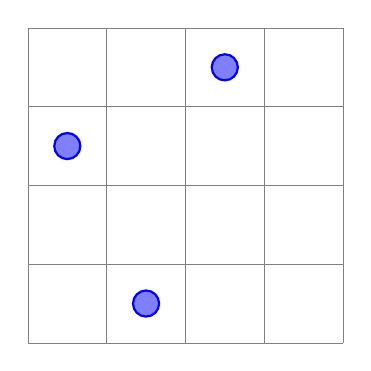
\begin{tikzpicture}[
simple/.style ={shape=circle, fill=grey!50},
blue/.style ={shape=circle, thick, draw=blue!100, fill=blue!50},
auto]
\draw[help lines] (0,0) grid (4,4);
%\fill (1cm,1.5cm) blue (5pt);
\node[blue] (a) at (0.5, 2.5) { };
\node[blue] (b) at (1.5, 0.5) { };
\node[blue] (c) at (2.5, 3.5) { };
\end{tikzpicture}

(partial solution for $n=4$)
\end{center}
\end{columns}

\end{frame}

%-------------------------------------------------------------
\begin{frame}[fragile]\frametitle{Mini-Project}

  Solve the ``cabbage - ferryman - goat - wolf'' problem:
  \begin{itemize}
  \item The four personalities are on the left side of a river and want to
    cross it
  \item Capacity of boat: 2
  \item Only the ferryman can row (possibly alone in the boat)
  \item May not remain without surveillance by the ferryman:
    \begin{itemize}
    \item Cabbage and goat
    \item Goat and wolf
    \end{itemize}
  \end{itemize}

\end{frame}

%-------------------------------------------------------------
\begin{frame}[fragile]\frametitle{Mini-Project}

  Transition graph for quadruples (cabbage, ferryman, goat, wolf)

  \begin{center}
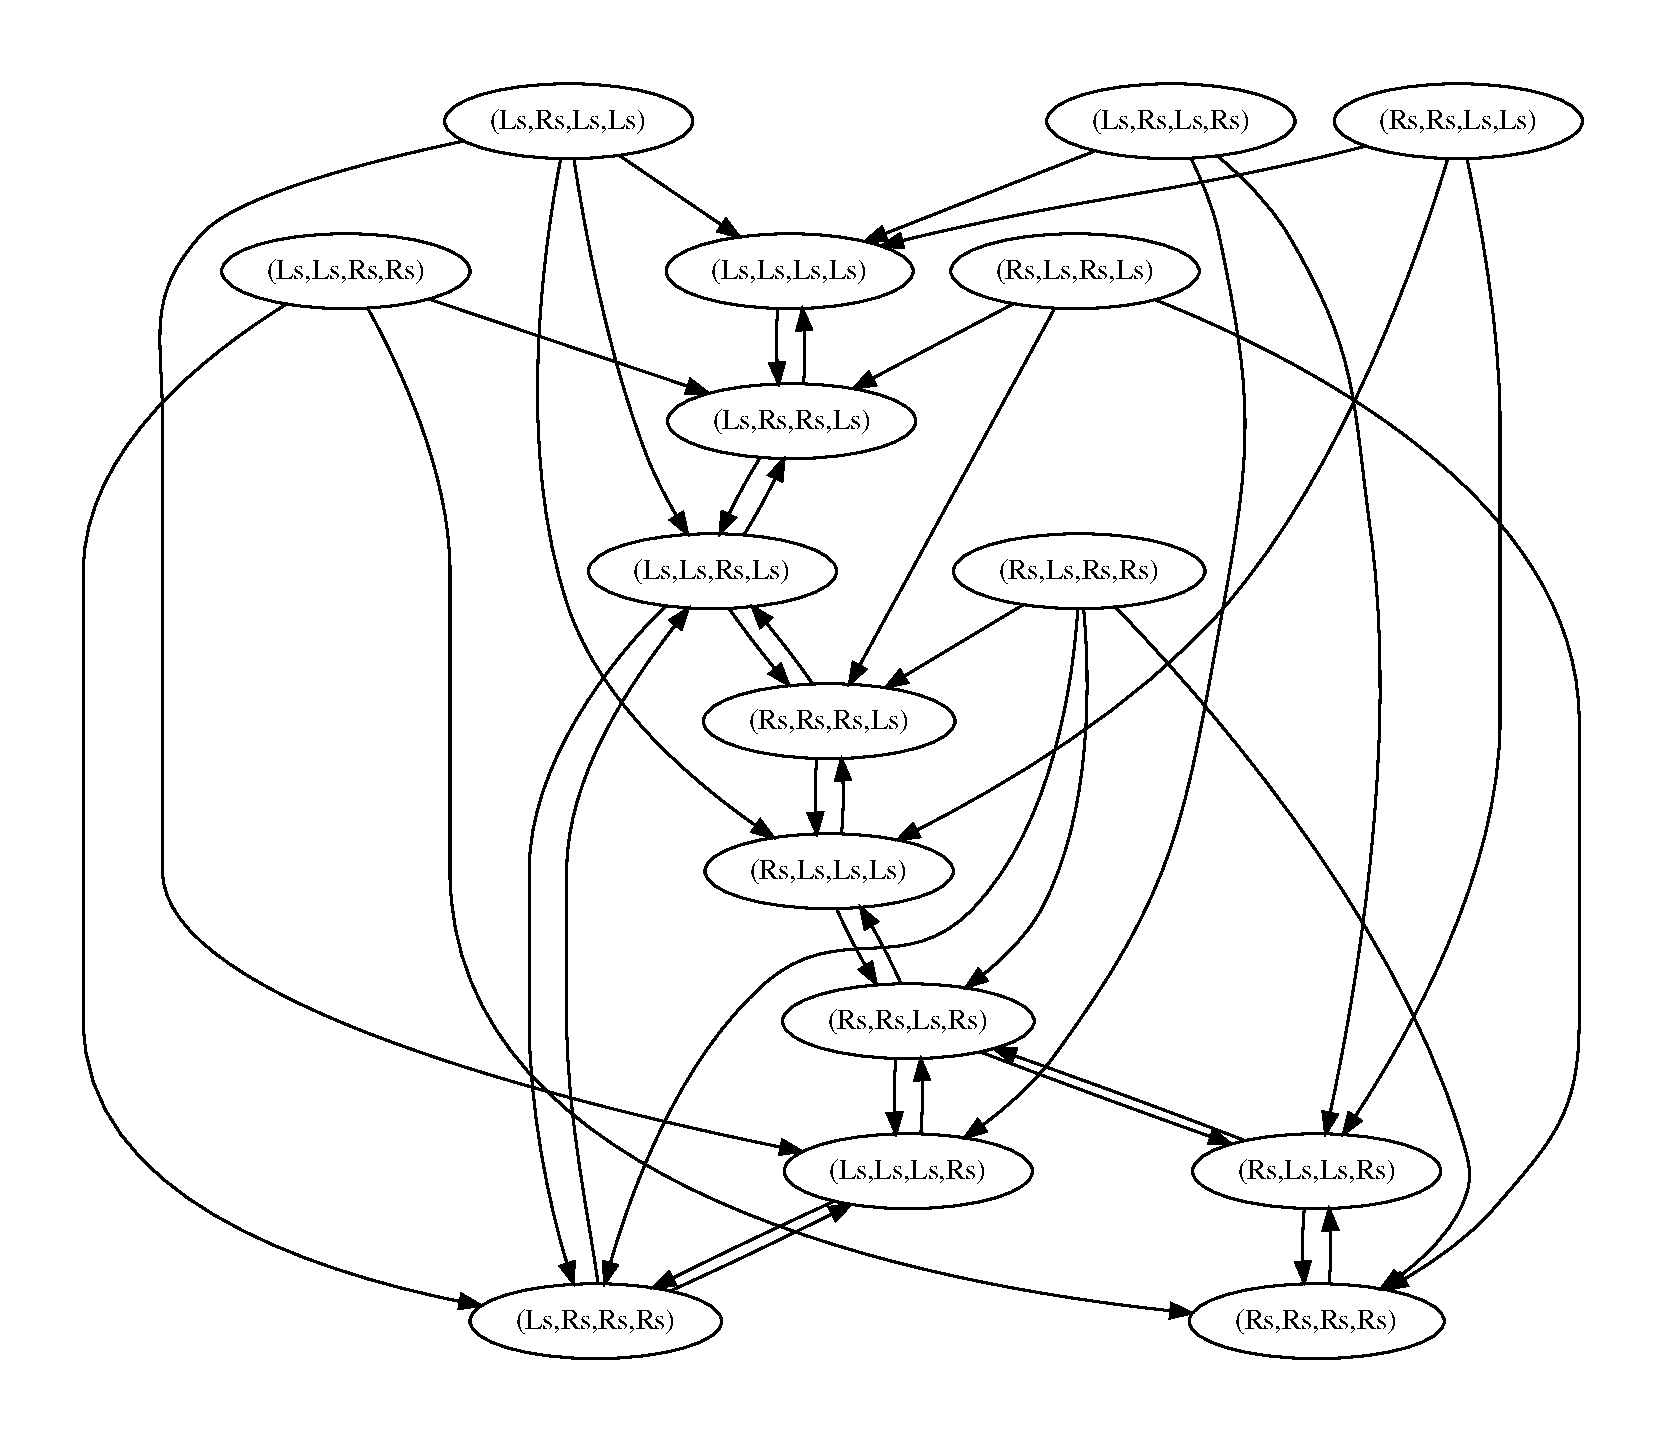
\includegraphics[scale=0.3]{Figures/river_crossing.pdf}
\end{center}


\end{frame}



%%% Local Variables: 
%%% mode: latex
%%% TeX-master: "main.tex"
%%% coding: utf-8-unix
%%% End: 
